\documentclass{article}\usepackage[]{graphicx}\usepackage[]{xcolor}
% maxwidth is the original width if it is less than linewidth
% otherwise use linewidth (to make sure the graphics do not exceed the margin)
\makeatletter
\def\maxwidth{ %
  \ifdim\Gin@nat@width>\linewidth
    \linewidth
  \else
    \Gin@nat@width
  \fi
}
\makeatother

\definecolor{fgcolor}{rgb}{0.345, 0.345, 0.345}
\newcommand{\hlnum}[1]{\textcolor[rgb]{0.686,0.059,0.569}{#1}}%
\newcommand{\hlsng}[1]{\textcolor[rgb]{0.192,0.494,0.8}{#1}}%
\newcommand{\hlcom}[1]{\textcolor[rgb]{0.678,0.584,0.686}{\textit{#1}}}%
\newcommand{\hlopt}[1]{\textcolor[rgb]{0,0,0}{#1}}%
\newcommand{\hldef}[1]{\textcolor[rgb]{0.345,0.345,0.345}{#1}}%
\newcommand{\hlkwa}[1]{\textcolor[rgb]{0.161,0.373,0.58}{\textbf{#1}}}%
\newcommand{\hlkwb}[1]{\textcolor[rgb]{0.69,0.353,0.396}{#1}}%
\newcommand{\hlkwc}[1]{\textcolor[rgb]{0.333,0.667,0.333}{#1}}%
\newcommand{\hlkwd}[1]{\textcolor[rgb]{0.737,0.353,0.396}{\textbf{#1}}}%
\let\hlipl\hlkwb

\usepackage{framed}
\makeatletter
\newenvironment{kframe}{%
 \def\at@end@of@kframe{}%
 \ifinner\ifhmode%
  \def\at@end@of@kframe{\end{minipage}}%
  \begin{minipage}{\columnwidth}%
 \fi\fi%
 \def\FrameCommand##1{\hskip\@totalleftmargin \hskip-\fboxsep
 \colorbox{shadecolor}{##1}\hskip-\fboxsep
     % There is no \\@totalrightmargin, so:
     \hskip-\linewidth \hskip-\@totalleftmargin \hskip\columnwidth}%
 \MakeFramed {\advance\hsize-\width
   \@totalleftmargin\z@ \linewidth\hsize
   \@setminipage}}%
 {\par\unskip\endMakeFramed%
 \at@end@of@kframe}
\makeatother

\definecolor{shadecolor}{rgb}{.97, .97, .97}
\definecolor{messagecolor}{rgb}{0, 0, 0}
\definecolor{warningcolor}{rgb}{1, 0, 1}
\definecolor{errorcolor}{rgb}{1, 0, 0}
\newenvironment{knitrout}{}{} % an empty environment to be redefined in TeX

\usepackage{alltt}
\usepackage{amsmath} %This allows me to use the align functionality.
                     %If you find yourself trying to replicate
                     %something you found online, ensure you're
                     %loading the necessary packages!
\usepackage{amsfonts}%Math font
\usepackage{graphicx}%For including graphics
\usepackage{hyperref}%For Hyperlinks
\usepackage[shortlabels]{enumitem}% For enumerated lists with labels specified
                                  % We had to run tlmgr_install("enumitem") in R
\hypersetup{colorlinks = true,citecolor=black} %set citations to have black (not green) color
\usepackage{natbib}        %For the bibliography
\setlength{\bibsep}{0pt plus 0.3ex}
\bibliographystyle{apalike}%For the bibliography
\usepackage[margin=0.50in]{geometry}
\usepackage{float}
\usepackage{multicol}

%fix for figures
\usepackage{caption}
\newenvironment{Figure}
  {\par\medskip\noindent\minipage{\linewidth}}
  {\endminipage\par\medskip}
\IfFileExists{upquote.sty}{\usepackage{upquote}}{}
\begin{document}

\vspace{-1in}
\title{Lab 10 -- MATH 240 -- Computational Statistics}

\author{
  Harrison Wolfe \\
  Colgate University  \\
  Math Department  \\
  {\tt hwolfe@colgate.edu}
}

\date{4/10/2025}

\maketitle

\begin{multicols}{2}\raggedcolumns
%\raggedcolumns % If your spacing gets messed up try uncommenting 
                % this line
\begin{abstract}
Confidence intervals are one of the most important statistical tools when trying to present data. They provide a range of values for which a certain percentage (typically around 95) of confidence intervals contain the true proportion or mean. There are several ways to create said intervals and some will be discussed below. 
\end{abstract}

\noindent \textbf{Keywords:} Confidence Intervals; Resampling; Point Estimates; Simulation

\section{Introduction}
In this lab we will be discussing different ways of calculating margin of error and therefore creating a confidence interval. Margin of error is the distance from a point estimate (mean of the survey data) to the bounds of each end of the confidence interval. For the first two methods, a Basic Simulation and Resampling, we will be calculating the margin of error given an example of a poll. This poll surveyed 1004 American's on the current state of the nation. They either said they were satisfied, dissatisfied, or that they did not have an opinion. In this survey it was found that 39 percent of participants were satisfied with the country however this number is much more useful when associated with a confidence interval to know how precise the estimate is. The other 2 methods, a more complicated simulation and the formula for margin of error, were done more generally for many different sample sizes and sample proportions values. 



\section{Basic Simulation}
One of the ways to conduct a confidence interval under the context of the polls example is using a basic simulation. In this simulation we ran 10,000 iterations of polling 1004 people with the condition that the true parameter was 0.39. Using this data we could create a confidence interval using the point estimate (mean of all proportions) from each sample giving us a margin of error of around 0.02988. If we double the sample size we were able to see that the margin of error decreases to 0.02117. This shows that margin of error is inversely correlated with sample size. Below we see histograms of each simulation and we can see that the second histogram has less variance than the first contributing to the smaller margin of error. The data that made these plots were made using \texttt{tidyverse} and the plots themselves were made using \texttt{ggplot2} \citep{tidyverse} \citep{ggplot}.

\begin{figure}[H]
\begin{center}
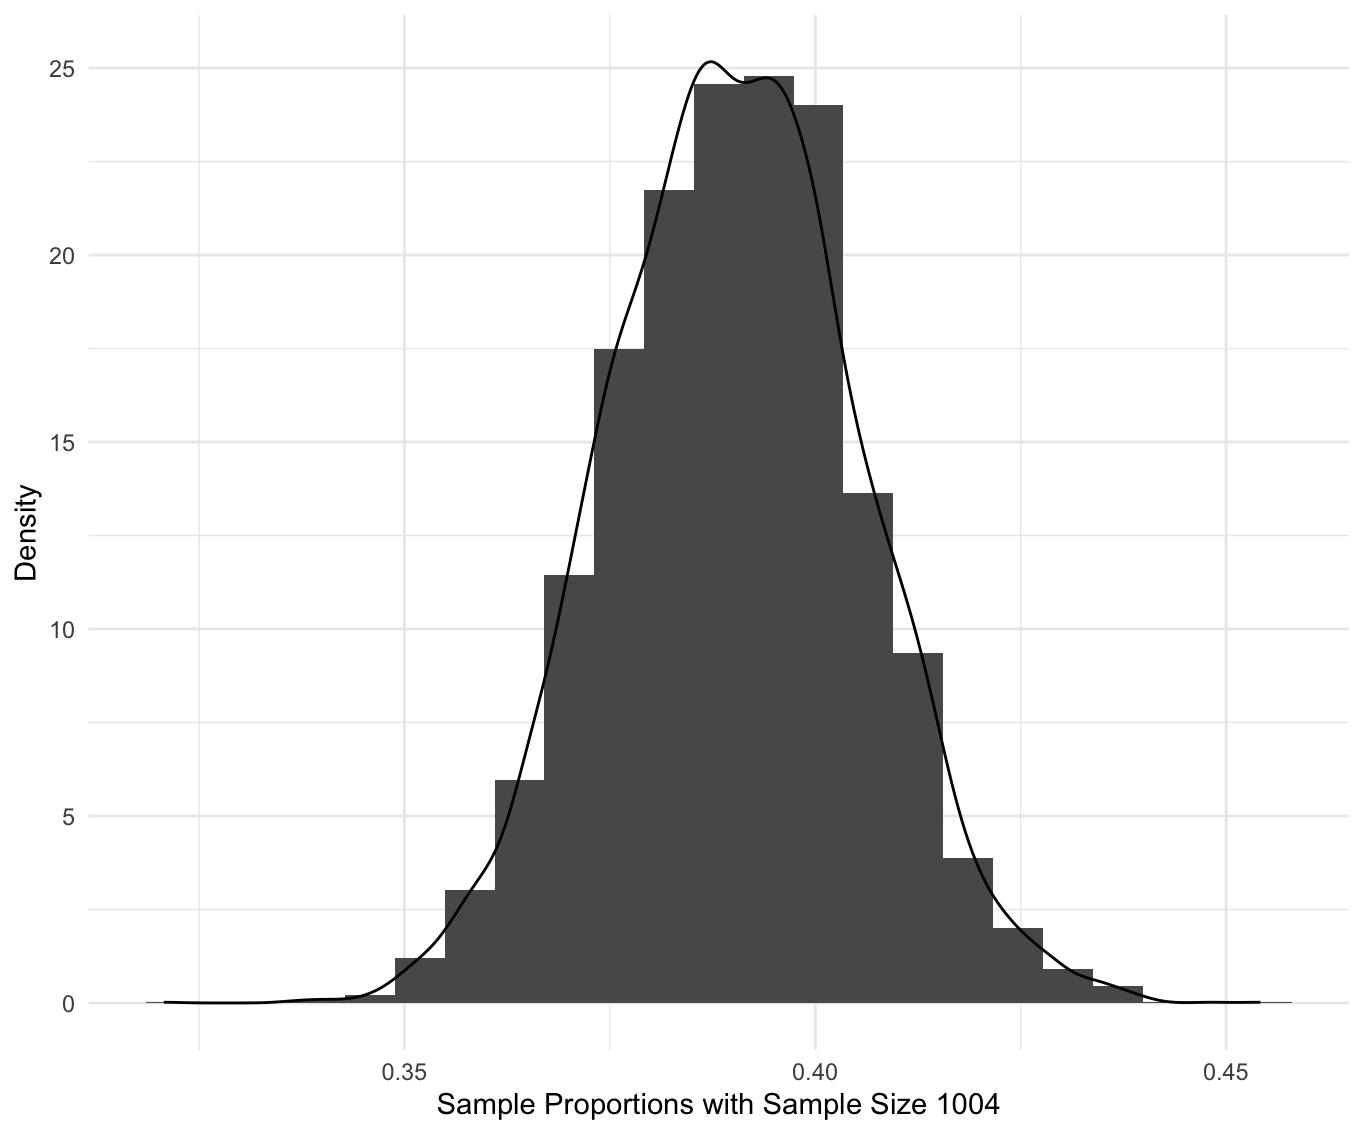
\includegraphics[scale=0.14]{first.png}
\caption{Basic Simulation with Sample Size 1004}
\label{Figure 1}
\end{center}
\end{figure}

\begin{figure}[H]
\begin{center}
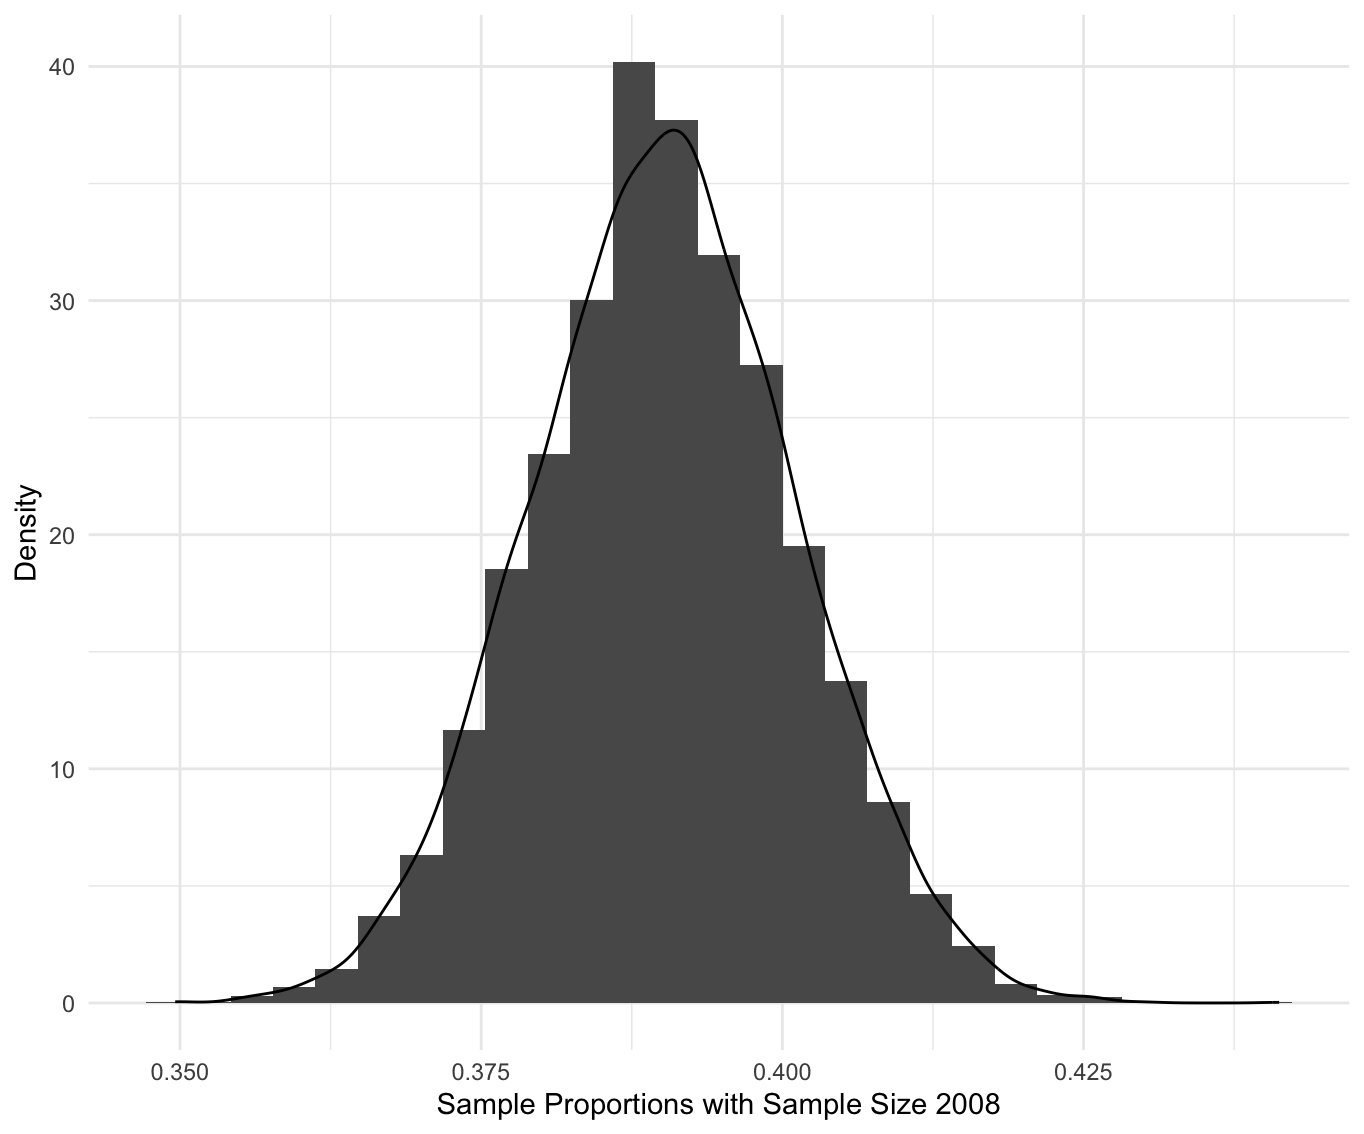
\includegraphics[scale=0.14]{second.png}
\caption{Basic Simulation with Sample Size 2008}
\label{Figure 2}
\end{center}
\end{figure}

\section{Resampling}

The second way we found margin of error was through resampling. Resampling is the process of taking a sample and taking random samples from the original sample with replacement and then calculaitng the statistics of interest. In this example we took the survey data regarding the satisfaction with the United States and resampled it 10,000 times. This process then gave us the ability to find a confidence interval with the middle 95 percent of the sample proportions which in turn gave us a margin of error. This margin of error was 0.02988. In Figure \ref{Figure 3} below we can see the variance of the distribution and the point estimate which was able to give us this margin of error found. 

\begin{figure}[H]
\begin{center}
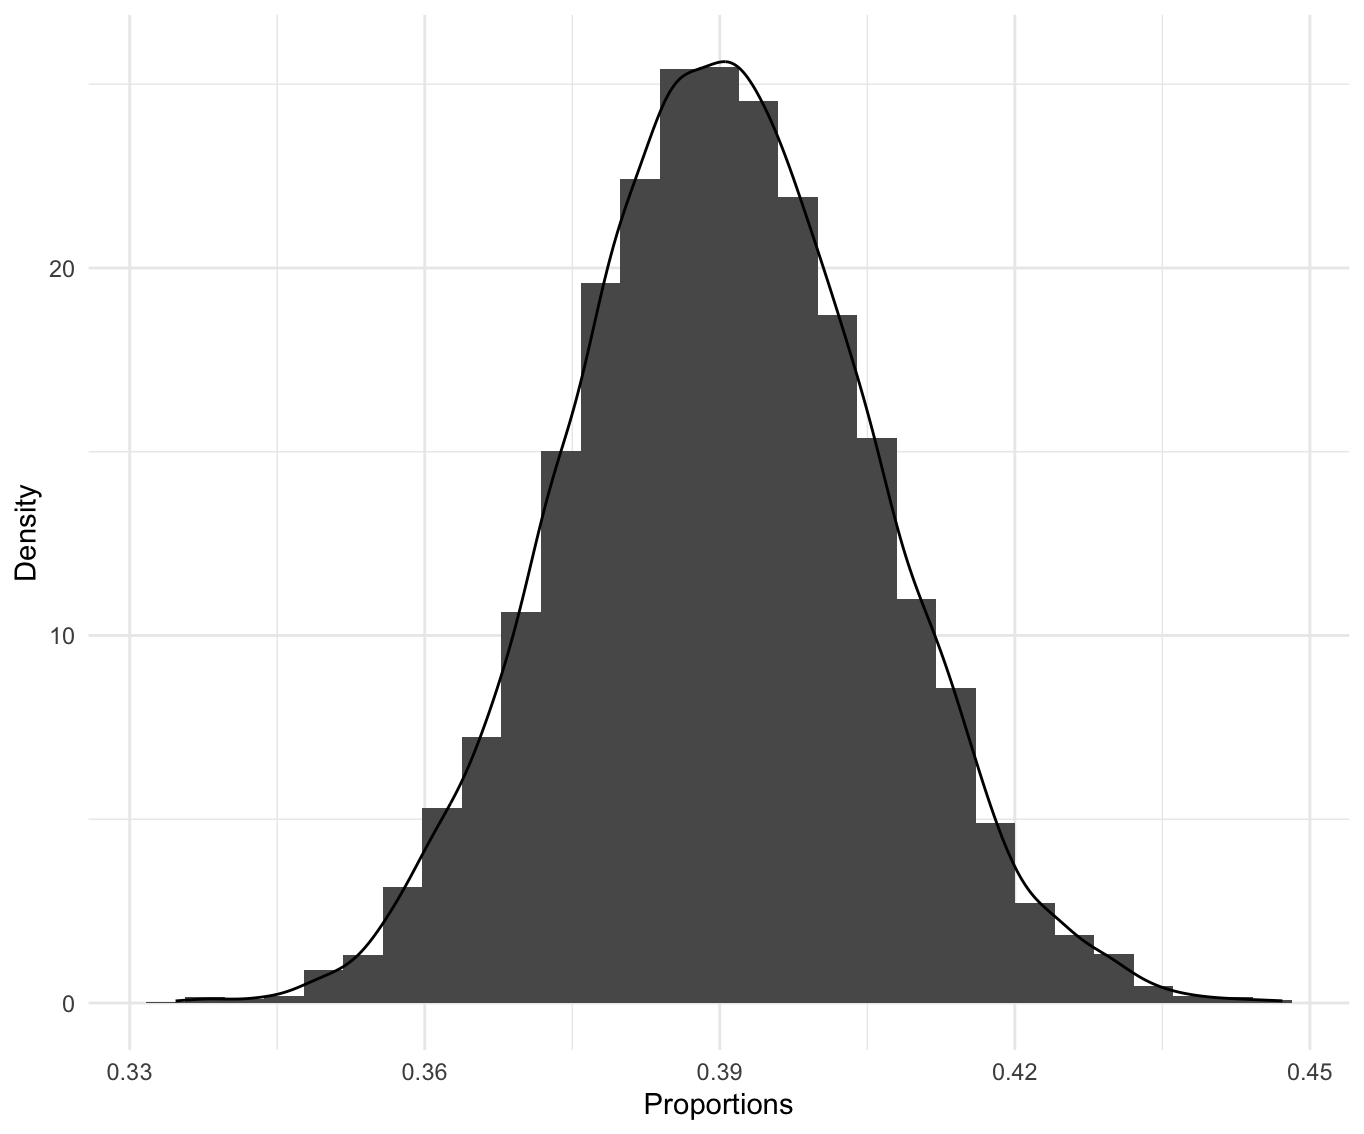
\includegraphics[scale=0.14]{third.png}
\caption{10,000 Resampled Sample Proportions}
\label{Figure 3}
\end{center}
\end{figure}

\section{Simulation over n and p}

In this simulation we simulated values with sample sizes going from 100 to 3000 by 10 for each proportion from 0.01 to 0.99 by 0.01. Using this information we were able to calculate a margin of error for each point. We found when the sample size was 1000 and the proportion was 0.39 (the survey data) the margin of error is 0.0305 which is similar to the resampling method. We can see in the Figure \ref{Figure 4} the way that margin of error changes with sample size and proportion. Margin of error grows when there is a low sample size and a proportion near 50 percent because that is given the most variance. However as we move in any direction away from these points we see that the margin of error decreases.

\begin{figure}[H]
\begin{center}
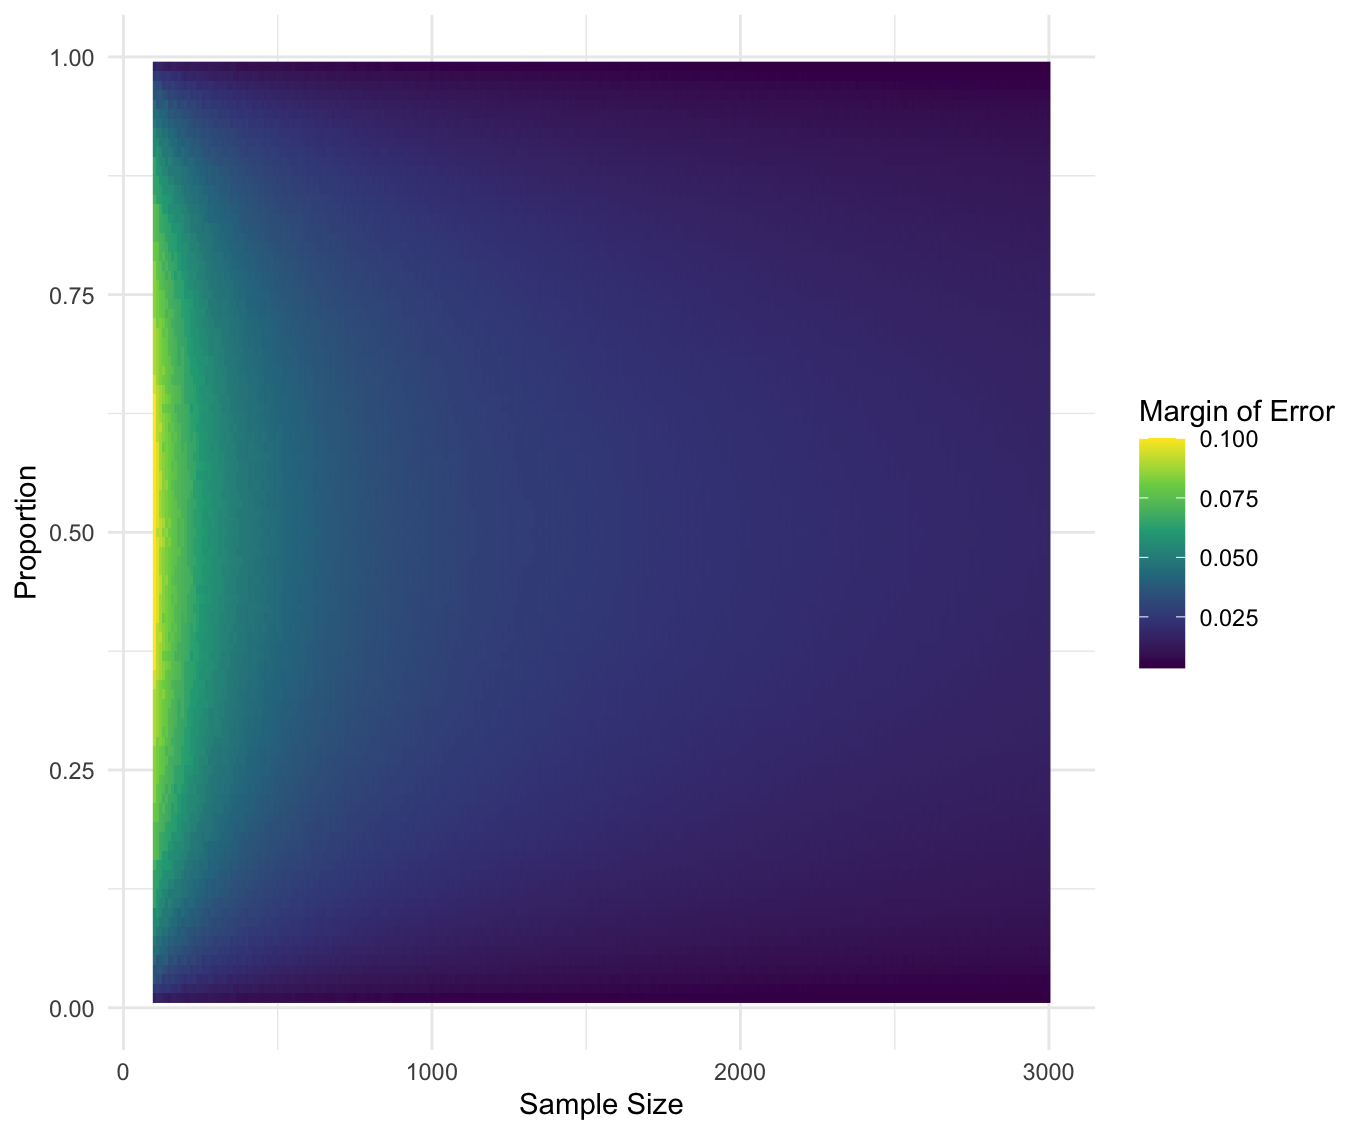
\includegraphics[scale=0.14]{fourth.png}
\caption{Margin of Error Based on Sample Proportion and Sample Size through Simulation}
\label{Figure 4}
\end{center}
\end{figure}

\section{Actual Margin of Error Calculation}
The final way we calculated margin of error was through a formula. This formula depends on our values for sample size, sample proportion, and the width of the confidence interval. Again for this method we calculated every margin of error for the same sample size and proportion values as the simulation. Through this we found that the margin of error for sample size 1000 and proportion 0.39 (like in the survey) was 0.03015. This value is again very similar to the resampling method and the simulation method. Again for this we plotted each point with each sample size and proportion in a heat map. Figure \ref{Figure 5} yields similar conclusions as Figure \ref{Figure 4}; it proves that margin of error generally is highest when sample size is low and the sample proportion is around 0.5 and as we escape from these points in the yellow region margin of error decreases. 

\begin{figure}[H]
\begin{center}
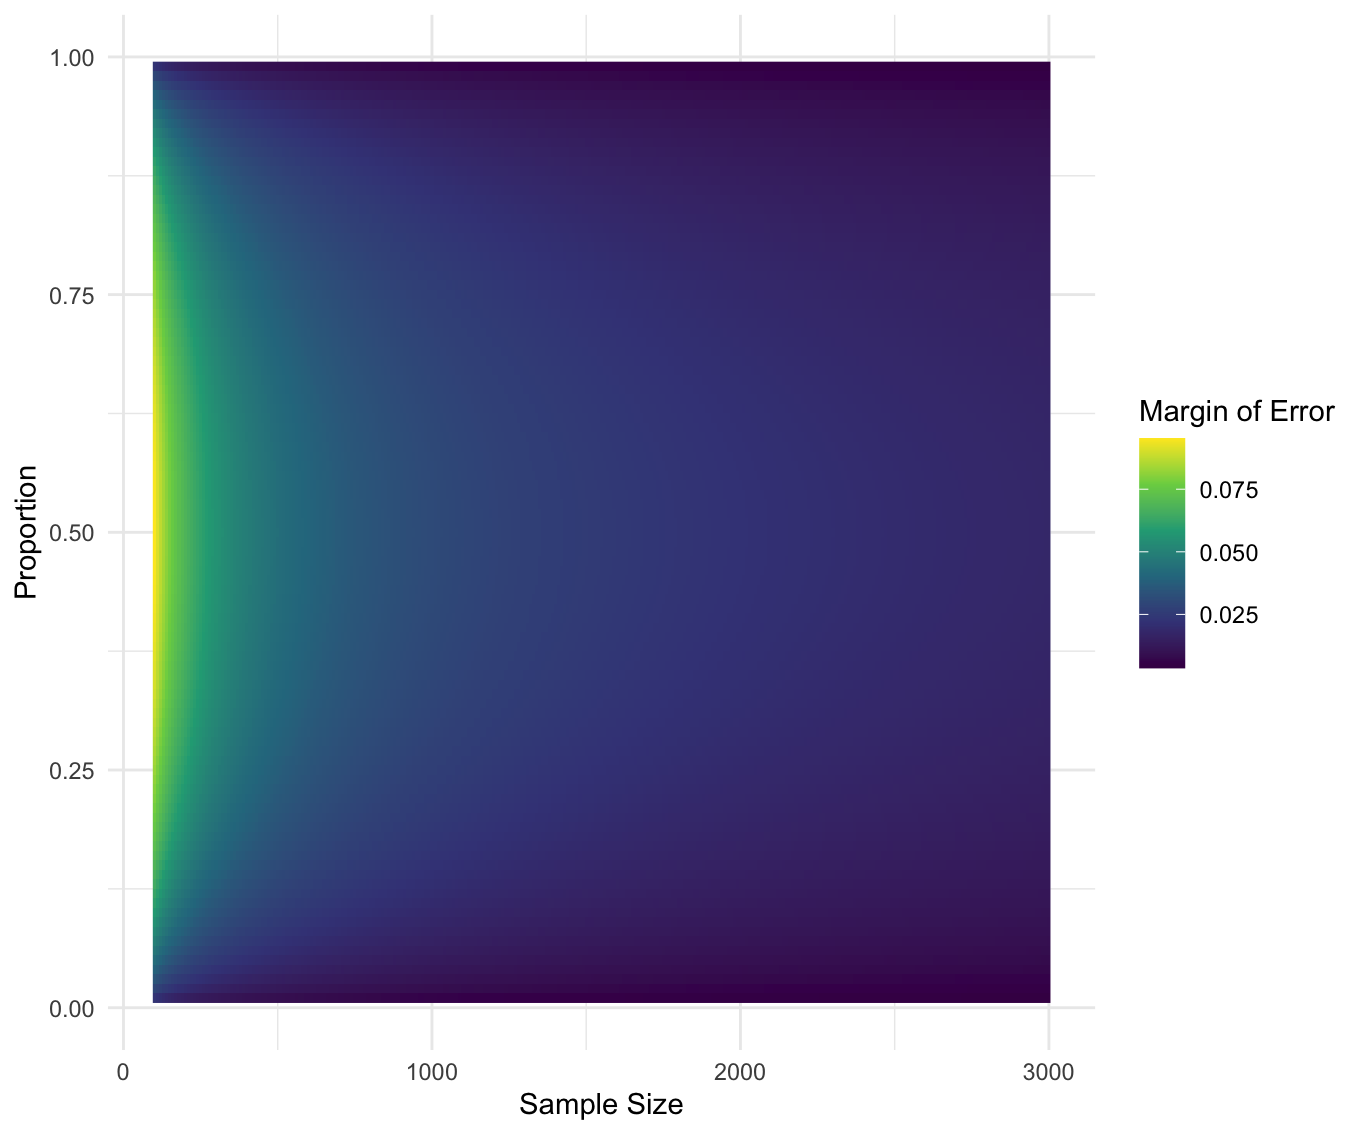
\includegraphics[scale=0.14]{fifth.png}
\caption{Margin of Error Based on Sample Proportion and Sample Size through Formula}
\label{Figure 5}
\end{center}
\end{figure}

\section{Conclusion}
As we can see with a basic simulation, resampling, simulating over sample size and sample proportion, and using the formula for margin of error given sample size and sample proportions we obtain values that are very close to each other given a specific example. 




%%%%%%%%%%%%%%%%%%%%%%%%%%%%%%%%%%%%%%%%%%%%%%%%%%%%%%%%%%%%%%%%%%%%%%%%%%%%%%%%
% Bibliography
%%%%%%%%%%%%%%%%%%%%%%%%%%%%%%%%%%%%%%%%%%%%%%%%%%%%%%%%%%%%%%%%%%%%%%%%%%%%%%%%
\vspace{2em}


\begin{tiny}
\bibliography{bib}
\end{tiny}
\end{multicols}


\end{document}
